\documentclass[12pt]{article}

\usepackage[letterpaper, margin=2cm]{geometry}
\usepackage{graphicx}
\usepackage[english]{babel}
\usepackage[utf8]{inputenc}
\usepackage{hyperref}
\usepackage[square,numbers,sort&compress]{natbib}
\usepackage{listings}
\usepackage{rotating}
\usepackage{placeins} %Force biblio at final document
\usepackage{epic,eepic}
\usepackage{rotating}
\usepackage{float}
\usepackage{array}
\usepackage{afterpage}
\usepackage{amsmath,amsfonts,amssymb}
\usepackage{booktabs}
%\usepackage[T1]{fontenc}
%\usepackage{sectsty}
\usepackage{adjustbox}

%opening
\title{Supplemental information \#2: A new strategy to characterize the domain 
architecture structure of proteins of the innate inmune system in tunicate 
species}
\author{Cristian A. Velandia-Huerto*, Ernesto Parra, Federico D. 
Brown, Adriaan Gittenberger, \\ Peter F. Stadler and Clara I. 
Berm\'{u}dez-Santana}
\begin{document}

\maketitle

%\begin{abstract}
%\end{abstract}

\section*{Golden Standard properties}

Golden Standard Group ($\boldsymbol{\mathfrak{G}}$) is composed with immune system sequences annotated in immune-specific databases (Insect Innate Immunity Database (IIID) and ImmuneDB). From the first one have been retrieved sequences from $5$ species of insects: (\textsl{Nasonia vitripennis}, \textsl{Apis mellifera}, \textsl{Drosophila melanogaster}, \textsl{Anopheles gambiae} and \textsl{Acyrthosiphon pisum}). For the second one,  additional sequences from mouse and human. All the detailed steps to retrieve the immune system sequences are described on the main text. Table \ref{tab:start} describes the number of sequences that have been annotated in those immune system databases. At the same time, complete annotation from the latter species have been retrieved from \texttt{Ensembl} in order to compare the percentage of proteins that are annotated as Immune System proteins by the referenced databases. 
First, all the reported proteins along the immune-system databases represented less than $3$\% in insect, while in mouse $\sim 9.32$\% and particulary in human a $\sim 36.90$\%. Also, the number of proteins that belong from human are the most frequent in $\boldsymbol{\mathfrak{G}}$, where represent a $84.74$\% followed by mouse sequences ($12.51$\%), while insects in total reported $2.75$\%.   

\begin{table}[ht!]
\begin{center}
\caption{Number of retrieved annotated proteins related to the Immune System. 
  The complete annotation of those proteins have been retrieved from \texttt{Ensembl}, including the relationships with their correspondend gene. The column \textsl{Ann. Proteins IS} are those proteins that have been reported on Immune system databases (\texttt{ImmuneDB} or \texttt{IIID}).} 
\label{tab:start}
\begin{tabular}{lp{2cm}p{2cm}p{2cm}p{2cm}p{1.5cm}l}
\toprule
\textbf{Specie} & \textbf{Complete Ann. Genes} & \textbf{Complete Ann. 
Proteins} & \textbf{Ann. Genes IS} & \textbf{Ann. Proteins IS} & \textbf{\%. Prot.} 
& \textbf{Database}\\
\midrule
\textit{A.\ pisum} & 26195 & 26195 & 65 & 81 (63) & $0.3092$ & IIID\\
\textit{A.\ gambiae} & 11840 & 13011 & 326 & 333 (326) & $2.5594$ & IIID\\
\textit{A.\ mellifera} & 10830 & 10830 & 105 & 106 (104) & $0.9788$ & IIID\\
\textit{D.\ melanogaster} & 12315 & 24557 & 181 & 242 (201) & $0.9855$ & IIID\\
\textit{N.\ vitripennis} & 13195 & 13253 & 350 & 368 (344) & $2.7767$ & IIID\\
\midrule
\textit{M.\ musculus} & 22090 & 55419 & 7043 & 5160 & $9.3109$ & 
ImmuneDB\\
\textit{H.\ sapiens} & 22413 & 94703 & 1803 & 34944 & $36.8985$ & 
ImmuneDB\\
\bottomrule
\end{tabular}
\end{center}
\end{table}

Once all the immune system proteins have been retrieved from \texttt{Ensembl}, the annotation of domains was organized later to define domain`s architectures in to define $\boldsymbol{\mathfrak{G}}$.

The arrangement of those protein domain architecures was performed independently for each annotation database (\texttt{Gene3d}, \texttt{PANTHER}, \texttt{Pfam},  \texttt{PIRSF}, \texttt{PRINTS}, \texttt{Prosite}, \texttt{SMART},\texttt{SUPERFAMILY} and \texttt{TIGRFAM}) generating the input architectures to be reduced by the \textsl{reduction system} (described in the main text). The direct effect performing this reduction of redundancy in the protein`s architecture is the reduction of the number of domains inside the proteins in $\boldsymbol{\mathfrak{G}}$ (Figure \ref{fig:groups}). The distribution of domains along $\boldsymbol{\mathfrak{G}}$ reported in all the protein databases that most of the domains comes from proteins that have been annotated 
on human. Additionaly, the distribution of domains along all the proteins shown that $75$\% of all proteins reported architectures with $\leq 2$ domains. At the same time, $\boldsymbol{\mathfrak{G}}$ also reported different 
distributions along the specific protein databases, in this case in the 
database \texttt{SMART} were reported the greatest number of domains inside a 
protein ($152$) and also, the database \texttt{Prosite} reported similar 
distributions. In overall, the greatest number of domains could be accessed. As an example in Table \ref{tab:greatestPfamComplete} is described the proteins that have the biggest number of domains, annotated with the \texttt{Pfam} database for each of the Gold Standard species. As expected, the annotation for the protein domains retrieved from \texttt{Ensembl} is related (when are avaliable) with the immune system. The annotation in general are related with detection proteins, like transmembrane receptors, or recognition of specific patterns, as lectins or directly Immunoglobulin domains. 

\begin{table}[ht!]
\begin{center}
\small
\caption{Highest number of protein domains reported in 
$\boldsymbol{\mathfrak{G}}$ for the \texttt{Pfam} database} 
\label{tab:greatestPfamComplete}
%\begin{tabular}{lp{2cm}p{1.5cm}p{1.5cm}p{1.5cm}p{1.5cm}p{1.5cm}p{1.5cm}p{1.5cm}
% p{1.5cm}}
\begin{adjustbox}{angle=90}
\begin{tabular}{lp{1.5cm}p{8.5cm}p{3.5cm}p{4.5cm}}
\toprule
\textbf{Specie} & \textbf{Numb.} &\texttt{Pfam} \textbf{Gene$|$ Protein}& 
\textbf{Most common Domain ACC., Name, (\%), No.}& \textbf{Annotation} \\
\midrule
\textit{A.\ pisum} & 7 & ACYPI008584$|$ACYPI008584-PA & PF01344, Kelch motif,  
$71.43$,5 & NA \\
\textit{A.\ gambiae} & 13 & AGAP000929$|$AGAP000929-PA & PF00084, Selectin, 
$84.61$, 11 &
C-type lectin (CTL) - selectin like \\
\textit{A.\ mellifera} & 34 & GB47938$|$GB47938-PA & PF00008, EGF-like 
domain, $26.47$, 9 & Gene CTL4 \\
\textit{D.\ melanogaster} & 27 & FBgn0243514$|$FBpp0301780 & PF02363, Cysteine 
rich repeat, $100.00$, 27 & Eater is a transmembrane receptor of the Nimrod 
family specifically expressed in hemocytes and required for the phagocytosis of 
Gram positive bacteria and the attachment of hemocytes to sessile 
niches.(\url{http://flybase.org/reports/FBgn0243514.html}) \\
\textit{N.\ vitripennis} & 41 & NV14569$|$NV14569-PA & PF00008, EGF-like 
domain, $56.10$, 23& 
NA \\
\midrule
\textit{M.\ musculus} & 50 & ENSMUSG00000040249$|$ENSMUSP00000044004 & 
PF00057, Low-density lipoprotein receptor domain class A, $60.00$, 30 & LDL 
receptor related protein 1 \\
\textit{H.\ sapiens} & 67 & ENSG00000154358$|$ENSP00000455507 & 
PF07679, Immunoglobulin I-set domain, $91.04$,61 & obscurin, cytoskeletal 
calmodulin and titin-interacting RhoGEF \\
\bottomrule
\end{tabular}
\end{adjustbox}
\end{center}
\end{table}


\begin{table}[ht!]
\begin{center}
\small
\caption{Highest number of protein domains reported in 
$\boldsymbol{\mathfrak{G}}$ for the \texttt{Pfam} database after the 
application of the reduction system, as explained in the main text, to 
generate protein architectures.} 
\label{tab:greatestPfamReduced}
\begin{adjustbox}{angle=90}
\begin{tabular}{lp{1.5cm}p{8.5cm}p{3.5cm}p{3.5cm}}
\toprule
\textbf{Specie} & \textbf{Number} &\texttt{Pfam} \textbf{Gene$|$ Protein}& 
\textbf{Most common Domain ACC., Name, (\%), No.} &  
\textbf{Annotation} \\
\midrule
\textit{A.\ pisum} & 5 & ACYPI007708$|$ACYPI007708-PA & All domains represented 
equally (1) in the arquitecture & NA \\
\textit{A.\ gambiae} & 7 & AGAP007237$|$AGAP007237-PA & PF07679, Immunoglobulin 
I-set domain, $28.57$, 2 & heme peroxidase 4 \\
\textit{A.\ mellifera} & 17 & GB47938$|$GB47938-PA & 
PF12661; PF07699; PF07645; PF02494; PF00754; PF00084 and PF00008, 
$11.76$, 2 & Gene CTL4 \\
\textit{D.\ melanogaster} & 14 & FBgn0029167$|$FBpp0075495 & PF08742, $35.71$, 
5 & Hemolectin (large multidomain protein produced by hemocytes and involved in 
the clotting reaction. ) \url{http://flybase.org/reports/FBgn0029167.html}\\
\textit{N.\ vitripennis} & 21 & NV14569$|$NV14569-PA & PF00008, EGF-like 
domain, $28.57$, 6 & NA \\
\midrule
\textit{M.\ musculus} & 16 & ENSMUSG00000027878$|$ENSMUSP00000078741 & PF00008, 
EGF-like domain, $37.50$, 6& Notch 2 \\
\textit{H.\ sapiens} & 32 & ENSG00000197558$|$ENSP00000485256 & PF01826, 
Trypsin Inhibitor like cysteine rich domain, $40.62$, 13 & 
SCO-spondin \\
\bottomrule
\end{tabular}
\end{adjustbox}
\end{center}
\end{table}

When the protein's architectures in $\boldsymbol{\mathfrak{G}}$ were analyzed 
along all the species, the distribution and the number of domains were 
calculated. The complete result is shown in Figure \ref{fig:groups_arch}, where 
all the information were analysed indenpendently by protein database and the 
distribution of protein architectures was calculated and its relation with the 
domain number. In this analysis were taken into account the number of 
architectures from $1$ because this set represents not only the proteins that 
have been only one domain but also, these ones that reported repetitions on the 
same domain and were collapsed after the reduction to one. In this set of $1$ 
domain, is posible to identify architectures that have been detected in a wide 
range of proteins along the annotation of the Golden Standard species; this 
pattern was detected for all the databases and also reported architectures that 
have been present in more than $1832$ proteins, as seen for the Immunoglobulins 
domain (Accession number: \texttt{2.60.40.10}). As shown in Figure 
\ref{fig:immunoglob}, this domain has been annotated in all of the 
species in \texttt{Ensembl} as: Immunoglobulin-like or 
Immunoglobulin-like-fold for the Gene3d database. Also, this region has another 
annotations for the same region by others protein domain databases, even 
including another protein domains and consequently generating another protein 
architectures. 

In general larger numbers in protein domains are not frequent in proteins in 
comparison to the lower ones, as seen when the range of the data is compared 
and also, supporting the pattern observed on Figure \ref{fig:groups}.

\begin{figure}[ht!]
\begin{center}
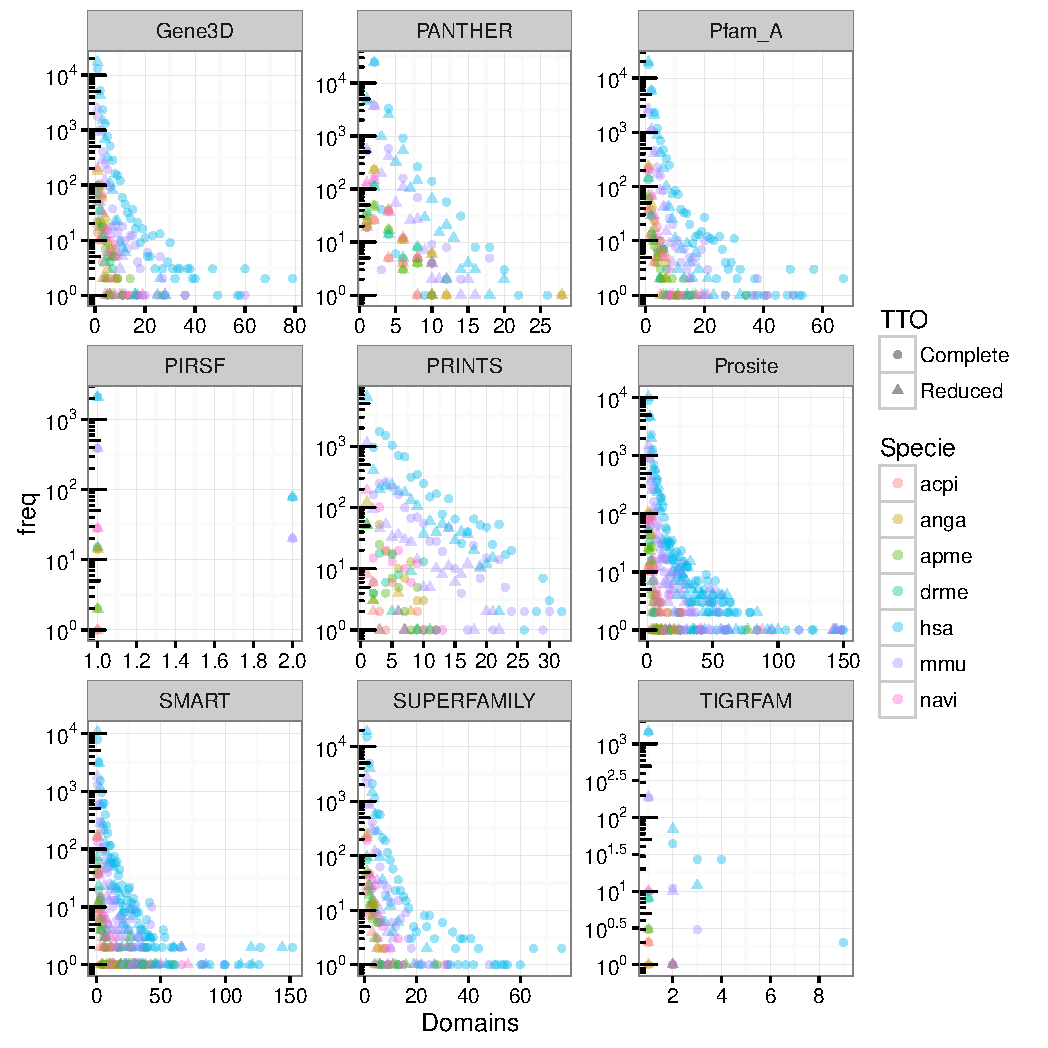
\includegraphics[scale=0.8]{distributionGroupsDomains}
\caption{Distribution of the number of domains in $\boldsymbol{\mathfrak{G}}$. 
\textbf{Acpi}: \textit{A. pisum}, \textbf{anga}: \textit{A. gambiae}, 
\textbf{apme}: \textit{A. mellifera}, \textbf{drme}: \textit{D. melanogaster}, 
\textbf{hsa}: \textit{H. sapiens}, \textbf{mmu}: \textit{M. musculus} and 
\textbf{Navi}: \textit{N. vitripennis}.}
\label{fig:groups}
\end{center}
\end{figure}


\begin{figure}[hb!]
\begin{center}
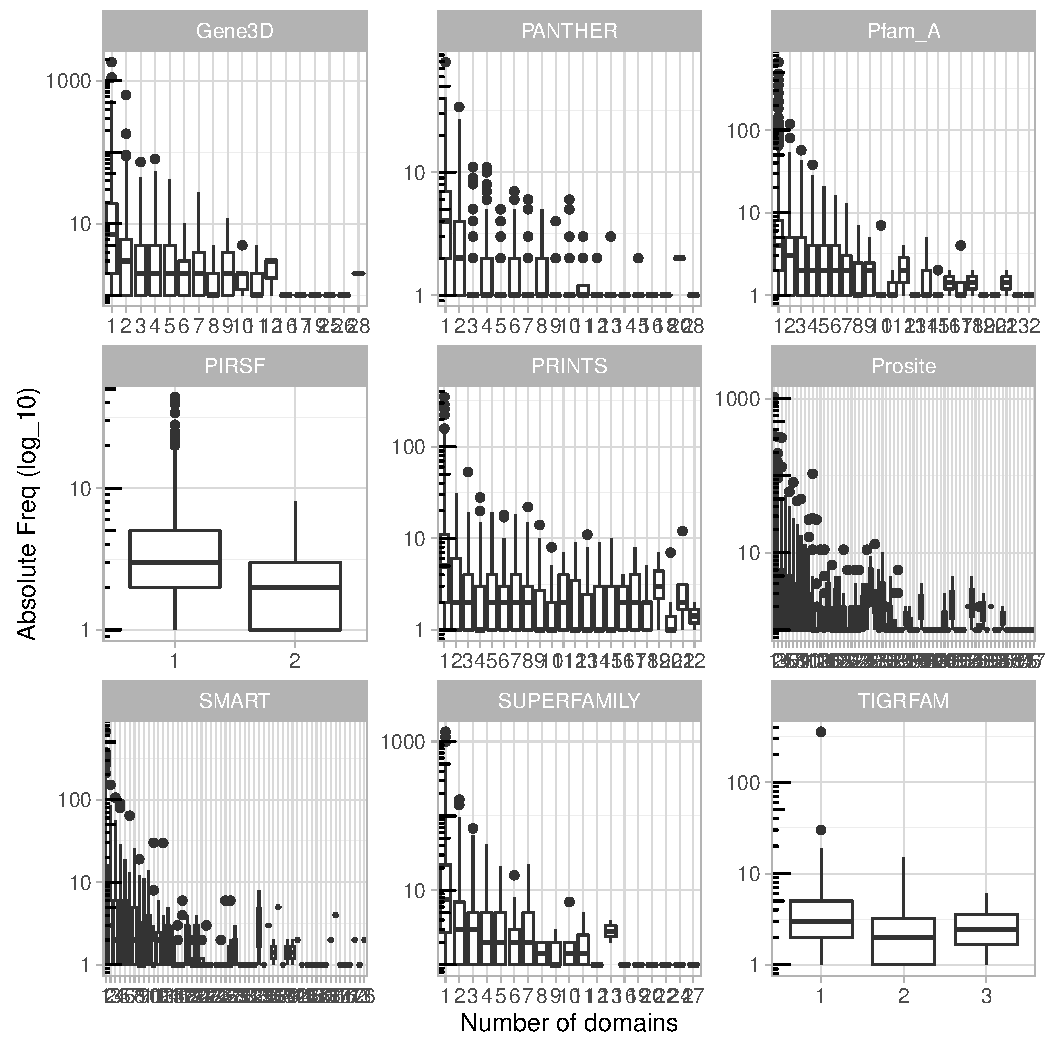
\includegraphics[scale=0.8]{architecturesDomains}
\caption{Distribution of protein architectures. The number of domains 
corresponds to the total number of annotated domains in the protein after the 
aplication of the reduction process and the Absolute Frequency is the counting 
of these architectures along all the organisms considered 
in $\boldsymbol{\mathfrak{G}}$.}
\label{fig:groups_arch}
\end{center}
\end{figure}

\begin{figure}[ht!]
\begin{center}
\includegraphics[scale=0.4]{most_freq}
\caption{Current annotation of the Immunoglobulin domain (2.60.40.10) along 
the Gold Standard Species: 
\textbf{Acpi}: \textit{A. pisum}, \textbf{apme}: \textit{A. mellifera}, 
\textbf{drme}: \textit{D. melanogaster}, 
\textbf{hsa}: \textit{H. sapiens}, \textbf{mmu}: \textit{M. musculus} and 
\textbf{Navi}: \textit{N. vitripennis}. In the current version of 
\texttt{Ensembl Metazoa} the annotation of \textbf{anga}: \textit{A. gambiae} 
for the protein \texttt{AGAP010083-PA} have been deprecated and redirected to 
the gen: \texttt{AGAP029053}.}
\label{fig:immunoglob}
\end{center}
\end{figure}

\end{document}
